\documentclass[11pt]{article}
\usepackage{graphicx}
\usepackage{hyperref}
\usepackage{appendix}
\usepackage{amsmath}
\usepackage{amsthm}
\usepackage{amssymb}
\usepackage{float}
\usepackage{multirow}
\usepackage{commath}
\usepackage{booktabs}
\usepackage{subcaption}
\renewcommand{\arraystretch}{1.2}
\newcommand{\code}[1]{\texttt{#1}}
\usepackage{siunitx}
\sisetup{detect-all}
\usepackage{listings}
\usepackage{color} %red, green, blue, yellow, cyan, magenta, black, white
\definecolor{mygreen}{RGB}{28,172,0} % color values Red, Green, Blue
\definecolor{mylilas}{RGB}{170,55,241}
\usepackage[a4paper,margin=20mm]{geometry}
\numberwithin{equation}{section}
\setlength{\parskip}{\baselineskip}
\setlength{\parindent}{0pt}
\hypersetup{
    colorlinks=true,
    linkcolor=black,
    filecolor=black,      
    urlcolor=black,
    citecolor=black
}
\urlstyle{same}
\begin{document}
\title{\textbf{UCL Mechanical Engineering 2021/2022}\\MECH0026 Coursework Two}
\author{Hasha Dar}
\date{\today}
\maketitle
\tableofcontents
\newpage
\listoffigures
\newpage
\section{Calculation and definition of the material properties from experimental data}
\subsection{Young's modulus}
The Young's Modulus of a material is a measure of stiffness of an elastic material. It has the following formula:
\begin{gather}
    E = \dfrac{\sigma}{\varepsilon} = \dfrac{\frac{F}{A}}{\frac{\Delta L}{L_0}}
\end{gather}
where $\sigma$ is the stress and $\varepsilon$ is the strain of the material. 

The Young's Modulus of the material can be calculated by finding the gradient of the elastic region on the engineering stress-strain curve. Using MATLAB, the following value for the slope of the curve was found:
\begin{gather}
    E = \SI{67.12}{\giga\pascal}   
\end{gather}
\subsection{Yield point}
The Yield Point is the stress at which a predetermined amount of permanent deformation occurs. To find the yield point of our material, we can use the offset method \cite{b1}. This is a recommended method of finding the yield point as stated in ASTM E8 \cite{b2}. The offset method involves plotting a line with gradient $E$ with an offset from the origin, typically in the range of 0.1\% - 0.2\% strain. Using MATLAB, we can find the yield stress and strain:
\begin{align}
    \sigma_y &= \SI{119.98}{\mega\pascal} \textrm{ at 0.2\% offset}\\
    \varepsilon_y &= \SI{3.78e-3}{} \textrm{ at 0.2\% offset}
\end{align}
\subsection{True stress-strain}
We can find the true stress and strain of our material by using the following equations:
\begin{gather}
    \sigma_t = \sigma_n e^{\varepsilon_n}\label{trueStress} \\
    \varepsilon_t = \ln\left(1 + \varepsilon_n\right) \label{trueStrain}
\end{gather}
The true stress-strain is a good fit until necking occurs, after which we have an instability in the material. After necking, three things happen:
\begin{itemize}
    \item volume does not remain constant.
    \item material is no longer homogeneous.
    \item material is no longer continuous.
\end{itemize}
Hence, \ref{trueStress} and \ref{trueStrain} represent the stress-strain of the damaged sample. 
\begin{figure}[H]
    \centering
    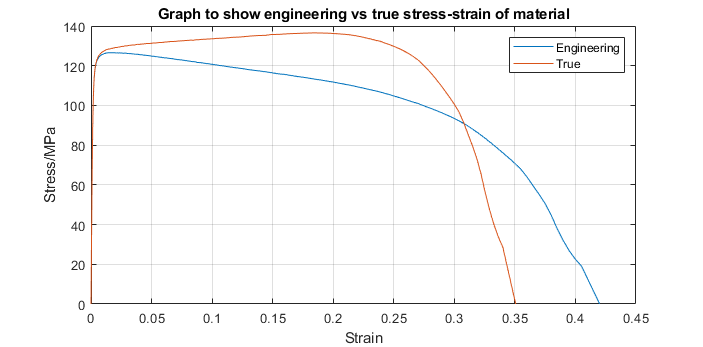
\includegraphics[width = \textwidth]{./img/engVsTrueStressStrain.png}
    \caption{Graph to show engineering vs true stress-strain response of material.}
    \label{engVsTrueStressStrainCurve}
\end{figure}
\subsection{Necking point/UTS}
To find the necking point, we need to find the ultimate tensile strength of our material, which can be found by indexing the largest stress value in our data.

Ultimate tensile strength (engineering):
\begin{gather}
    \sigma_{e,uts} = \SI{126.52}{\mega\pascal} \textrm{ at } \varepsilon = \SI{0.019}{}
\end{gather}
Ultimate tensile strength (true):
\begin{gather}
    \sigma_{t,uts} = \SI{136.51}{\mega\pascal} \textrm{ at } \varepsilon = \SI{0.186}{}
\end{gather}
We take the value from our true stress-strain curve as this accurately represents the stress-strain of our material until necking occurs.
\subsection{Effective stress-strain}
The effective stress-strain allows us to model the true undamaged stress-strain of the material. This is useful as ABAQUS requires this to model the behaviour of our material. This can be calculated by assuming a perfectly plastic response after the onset of necking:
\begin{gather}
    \widetilde{\sigma}_t = \begin{cases}
        \sigma_t & \textrm{for } \varepsilon_n \leq \varepsilon_{n,uts}\\
        \sigma_{n,uts}\left(1 + \varepsilon_n\right) & \textrm{for } \varepsilon_n > \varepsilon_{n,uts}
    \end{cases}\\
    \widetilde{\varepsilon}_t = \varepsilon_t
\end{gather}
A plot of the effective stress-strain curve is shown below.
\begin{figure}[H]
    \centering
    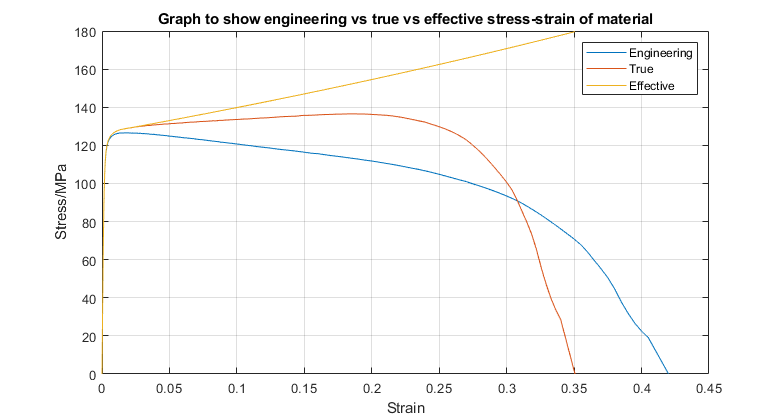
\includegraphics[width = \textwidth]{./img/engVsTrueVsEffectiveStressStrain.png}
    \caption{Graph to show engineering vs true vs effective stress-strain response of material.}
    \label{engVsTrueVsEffectiveStressStrainCurve}
\end{figure}
\subsection{Damage parameter}
The damage of the material is a measure of the area of voids in a material. The effective true stress can be written in terms of the damage variable:
\begin{align}
    \widetilde{\sigma}_t = \frac{F}{A-A_D} = \frac{F}{A\left(1 - \frac{A_D}{A}\right)} = \frac{\sigma_t}{1 - D}
\end{align}
Rewriting Hooke's Law:
\begin{gather}
    \widetilde{\sigma}_t = E \varepsilon_t \rightarrow \sigma_t = E\left(1-D\right)\varepsilon_t
\end{gather}
ABAQUS requires that damage evolution be inputted as a function fo the equivalent plastic displacement after necking, as strains are mesh dependent.
\begin{gather}
    \overline{u}_{pl} = L*\left(\overline{\varepsilon}^{pl}_t - \overline{\varepsilon}^{pl}_{t,uts}\right)
\end{gather}
where $L$ is the element size, $\overline{\varepsilon}^{pl}_t$ is the equivalent plastic strain and $\overline{\varepsilon}^{pl}_{t,uts}$ is the equivalent true plastic strain at the onset of necking. 
\section{Description of FEM setup}
\subsection{Boundary and loading conditions}
The test sample was sketched and modelled in ABAQUS.
\begin{figure}[H]
    \centering
    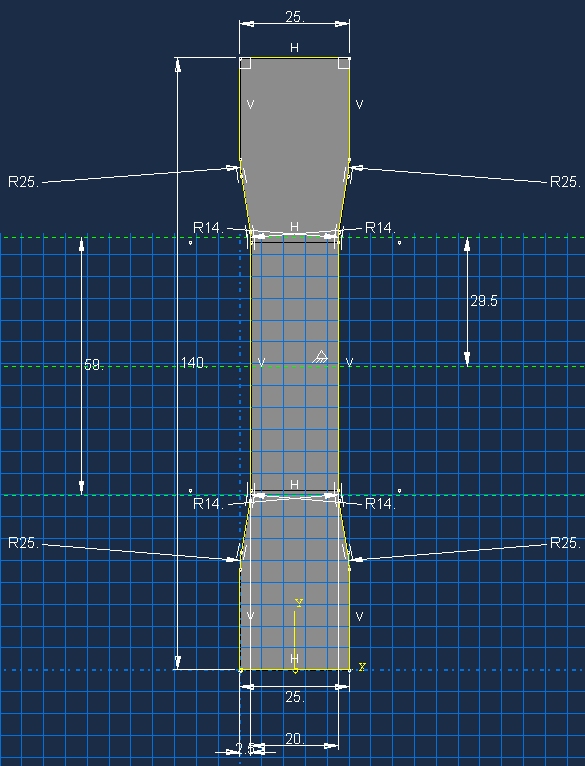
\includegraphics[width = 0.7\textwidth]{./img/Sketch1.png}
    \caption{Sketch of test sample in ABAQUS.}
    \label{sampleSketch}
\end{figure} 
The following boundary and loading conditions were applied:
\begin{itemize}
    \item Bottom fixed in U1, U2, UR3.
    \item Top displaced in U2 10 units upwards and fixed in U1 and UR3.
\end{itemize}
\subsection{Element type and justification}
Since we are looking at a relatively thin plate undergoing stresses in the $x$- and $y$- directions, we can model the plate in a 2D configuration with thickness \SI{1.5}{\milli\m}. We can assume here that through thickness stresses are zero and the in-plane stresses are constant through thickness in the component. We can make this assumption due to the relatively small thickness of the plate in comparison to its other dimensions. Hence, we can choose to focus on plane stress for our simulation.
\begin{gather}
    \sigma_z = \sigma_{zx} = \sigma_{zy} = \varepsilon_{zx} = \varepsilon_{zy} = 0
\end{gather}
\subsection{Material models employed}
A new material (labeled `alu') was created in ABAQUS with the following properties:
\begin{itemize}
    \item Elastic
    \begin{itemize}
        \item Young's modulus: \SI{67114.97}{\giga\pascal} (MATLAB variable \texttt{`YM'})
        \item Poission's ratio: 0.3 (given)
    \end{itemize}
    \item Plastic
    \begin{itemize}
        \item Yield stress and plastic strain: tabular data (MATLAB variable \texttt{`plasticYield'})
    \end{itemize}
    \item Ductile damage
    \begin{itemize}
        \item Fracture strain: 0.015 (MATLAB variable \texttt{`equivTrueUTSPlasticStrain'})
        \item Stress triaxiality: 0.333 (given)
        \item Strain rate: 0
    \end{itemize}
    \item Damage evolution: type - displacement, softening - linear, displacement at failure: 0.3212 (MATLAB tabular data \texttt{`equivPlasticDisp'})
\end{itemize}
\subsection{Mesh configuration and convergence}
As our model involves variables which are sensitive to mesh size, choosing an appropriate mesh size is important to ensure accurate results. The Von-Mises stress was used as a convergence criterion: 
\newpage
\begin{thebibliography}{00}
    \bibitem{b1} Illinois Tool Works, (2022) `Offset Yield Strength' \url{https://www.instron.com/en-gb/our-company/library/glossary/o/offset-yield-strength} Accessed: 01/03/22
    \bibitem{b2} ASTM, (2022) `Standard Test Methods for Tension Testing of Metallic Materials' \url{https://www.astm.org/e0008_e0008m-21.html} Accessed: 01/03/22
\end{thebibliography}
\end{document}